\section{Calibration}\label{sec:calibration}

\subsection{Hyperparameter Tuning}\label{subsec:hyperparameter-tuning}

In the \emph{SynBA score} formula defined in \ref{subsubsec:transformation}, the weights $\lambda_1, \lambda_2, \lambda_3$ are hyperparameters that need to be tuned. 
Those values are used to balance the three components of the formula, and they should sum up to 1.

The calibration of the hyperparameters is performed by using the \emph{HypeOpt} \cite{conf/icml/BergstraYC13} library, which is a hyperparameter optimization library for Python. 
should be chosen in order to maximize the performance of the model.
TPE \cite{bergstra2011algorithms} is a default algorithm for the \emph{HypeOpt}. It uses the Bayesian approach for optimization. At every step, it is trying to build a probabilistic model of the function and choose the most promising parameters for the next step. Generally, this type of algorithms works like this:
\begin{enumerate}
    \item generate a random initial point  $x^*$ 
    \item calculate  $F(x^*)$
    \item using the history of trials try to build the conditional probability model  $P(F|x)$
    \item choose  $x_i$  that according to  $P(F|x)$  will most probably result in better  $F(x_i)$
    \item compute the real value of the  $F(x_i)$ 
    \item repeat steps 3-5 until $i > max\_eval$
\end{enumerate}

Since \emph{HypeOpt} doesn't support multi-objective optimization, we have to define a single objective function to ensure that the method performs well.
So we designed the following loss function that the optimization algorithm aims to minimize:
\begin{multline}
    loss = - ( avg\_sbert\_similarity * (1 - contraddiction\_rate) ) + penalty \\
    \qquad \text{where} \quad penalty = 0.35 *  \frac{failed\_attacks}{successful\_attacks + failed\_attacks}\\
\end{multline}

It combines two quality metrics defined in \ref{subsec:quality-metrics} and penalizes the attacks that frequently fail to generate adversarial examples.
A particular version of the contradiction rate metric is used, which instead of comparing the whole original and perturbed text, it splits the text into sentences and counts as contradiction the samples containing at least a pair of sentences that are contradictory.

The search space of the hyperparameters is defined by the combination of three decimal values $\in [0, 1]$ that sum up to 1.

The optimization algorithm performed 50 trials, attacking a fine-tuned BERT model for sentiment analysis using 500 samples from \emph{yelp-polarity} \cite{zhang2015characterlevel} dataset (which is on purpose different from benchmark datasets used for evaluation in \ref{sec:evaluation-framework}).
The best hyperparameters are chosen as the ones that minimize the loss function.
Table \ref{tab:3_5_hyperparameter_tuning} shows the ten optimal results of the optimization process.

\begin{table}[h]
    \footnotesize
    \centering
    \begin{tabular}{|c|c|c|c|c|c|c|c|c|c|}
        \hline
        $\lambda_1$ & $\lambda_2$ & $\lambda_3$ &  Succ &  Fail &  Skip &  Contradiction rate &  SBERT similarity &  Loss \\
        \hline
        \hline
        0.284 & 0.107 & 0.608 & 431.0 &  58.0 &  11.0 &  0.501 &  0.915 &  -0.41507 \\
        0.247 & 0.104 & 0.648 & 431.0 &  58.0 &  11.0 &  0.501 &  0.915 &  -0.41507 \\
        0.488 & 0.463 & 0.047 & 356.0 & 133.0 &  11.0 &  0.441 &  0.908 &  -0.41237 \\
        0.365 & 0.057 & 0.576 & 429.0 &  60.0 &  11.0 &  0.503 &  0.916 &  -0.41230 \\
        0.238 & 0.215 & 0.545 & 430.0 &  59.0 &  11.0 &  0.505 &  0.915 &  -0.41069 \\
        0.323 & 0.150 & 0.526 & 431.0 &  58.0 &  11.0 &  0.506 &  0.915 &  -0.41049 \\
        0.376 & 0.116 & 0.507 & 428.0 &  61.0 &  11.0 &  0.505 &  0.916 &  -0.40975 \\
        0.495 & 0.486 & 0.018 & 356.0 & 133.0 &  11.0 &  0.444 &  0.907 &  -0.40909 \\
        0.487 & 0.480 & 0.032 & 357.0 & 132.0 &  11.0 &  0.445 &  0.907 &  -0.40890 \\
        0.008 & 0.215 & 0.775 & 399.0 &  90.0 &  11.0 &  0.489 &  0.924 &  -0.40774 \\
        \hline
    \end{tabular}
\caption{Hyperparameter tuning results for SynBA score weights}
\label{tab:3_5_hyperparameter_tuning}
\end{table}

%**************************************************************

\subsection{Transformation ranking calibration}\label{subsec:transformation-ranking-calibration}
The candidate pool range $k$ is another hyperparameter used in the SynBA transformation.
Intuitively, increasing candidate size led to a higher attack success rate, although, a larger 
$k$ would result in less semantic similarity.

So it is not trivial to choose the best value for $k$. 
We selected an arbitrary value of $k=30$ and we computed a set of additional metrics:

\begin{itemize}
    \item \textbf{Average max rank} - the maximal transformation ranking that is applied to the input averaged over all the samples;
    \item \textbf{Average min rank} - the minimal transformation ranking that is applied to the input averaged over all the samples;
    \item \textbf{Average mean rank} - the mean transformation rankings that are applied to the input averaged over all the samples;
    \item \textbf{Average std rank} - the standard deviation of the transformation rankings that are applied to the input averaged over all the samples;
    \item \textbf{Average mean reciprocal rank} - the \acrshort{mrr} metric averaged over all the samples.
\end{itemize}
The MRR measures how far down the ranking of the perturbed candidate is. It is calculated as:

\begin{equation}
    \text{MRR} = \frac{1}{|C|} \sum_{c \in C} \frac{1}{rank(c)} \\
\end{equation}
where $C$ is the candidate pool of $k$ tokens. 


Evaluating the rank metrics on a fine-tuned BERT model for sentiment analysis using 1000 samples from \emph{yelp-polarity} dataset, 
we obtained the following results:
\begin{itemize}
    \item Average max rank: 23.12
    \item Average min rank: 3.31
    \item Average mean rank: 11.69
    \item Average std rank: 6.83
    \item Average mean reciprocal rank: 0.20
\end{itemize}

Those results evidence that there is no need to increase the candidate pool size, since the average max rank is lower than the chosen threshold.

The final version of SynBA with all the parameters tuned is reported in Figure \ref{fig:3_synba_components},
highlighting the component division of the TextAttack framework.

\begin{figure}[h]
    \centering
    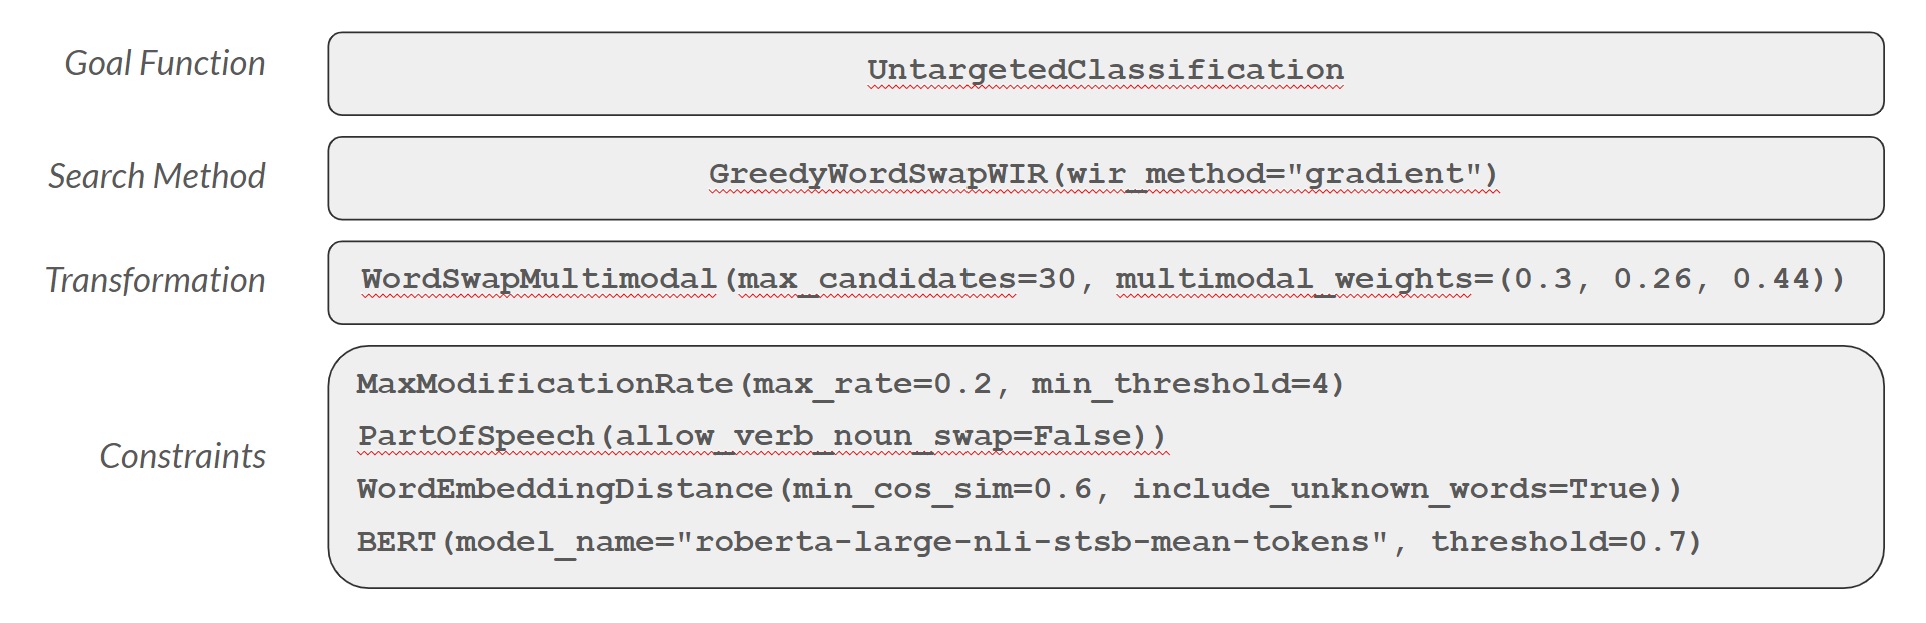
\includegraphics[width=0.9\linewidth]{images/3_synba_components.png}
    \caption{SynBA components}
    \label{fig:3_synba_components}
\end{figure}
%**************************************************************

